\section{SMURF Examples}

In this section, we provide two examples that use a variety of language features in SMURF.

\subsection{Simple Example}
The simple SMURF program shown in Figure~\ref{fig:example1} first defines the pitch classes for the prime row in line 1. Using the prime row as a base, the program creates a score with a single measure using the notes generated by transposing the prime row by three semitones (line 2), inverting the resulting transposed row (line 3), and then reversing the inverted row from the prior step (line 4). Lines 2-4 use the \emph{trans, inver, and rev} library routines to apply transposition, inversion, and reversal to a list, respectively. Line 5 invokes a library routine called \emph{rowToNotes} that converts each pitch class in a tone row to a list of notes given beat and register value mappings for each pitch class in the tone row. For simplicity, all the notes in this example are quarter notes (4) in register 0. Line 6 defines a measure using the first two notes in the list of notes returned in line 5; the second half of the measure consist of two rest quarter notes in register 0.  Line 7 uses the keyword \textbf{genScore} along with the measure defined in the prior line as an argument. The compiler translates the keyword \textbf{genScore} down to C+OpenGL code to create a score sheet based on the given list of measures.     

\begin{figure}
  \centering
  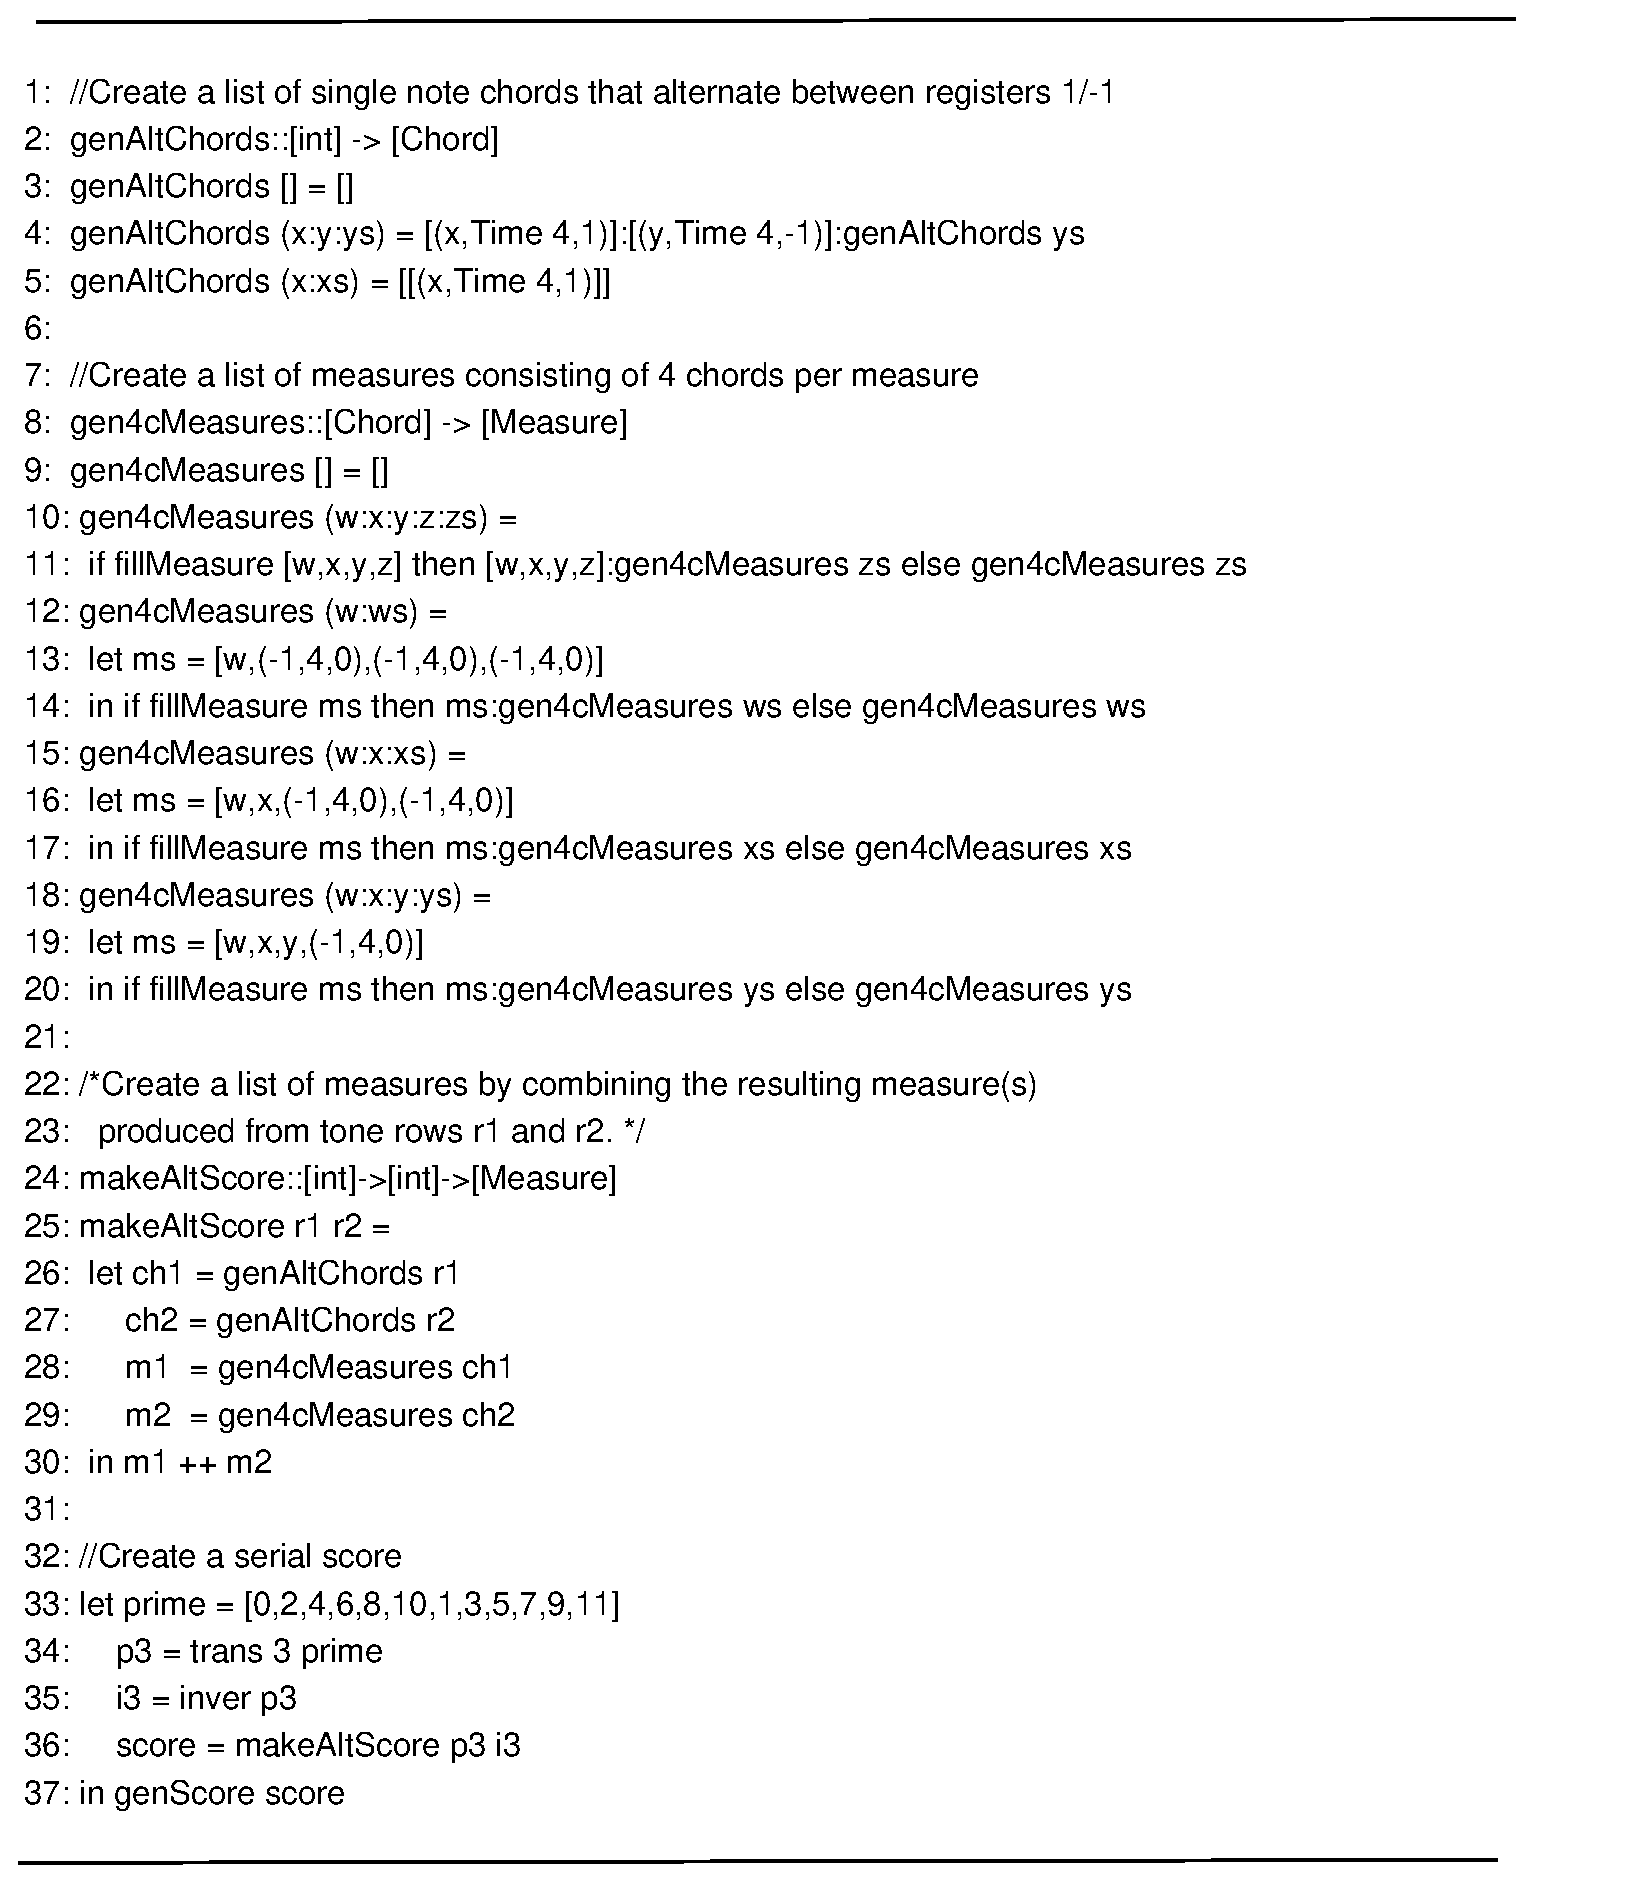
\includegraphics[width=\textwidth]{figures/example1}
  \caption{Simple SMURF example code. The code uses the trans, inver, and rev library routines to generate a tone row that is then used to create notes, a measure, and then finally a score.}
  \label{fig:example1}
\end{figure}

\subsection{Second Example}

The example code presented in Figure~\ref{fig:example2} shows how to define functions, use keywords, use types, and apply operators in SMURF. 

\begin{figure}
  \centering
  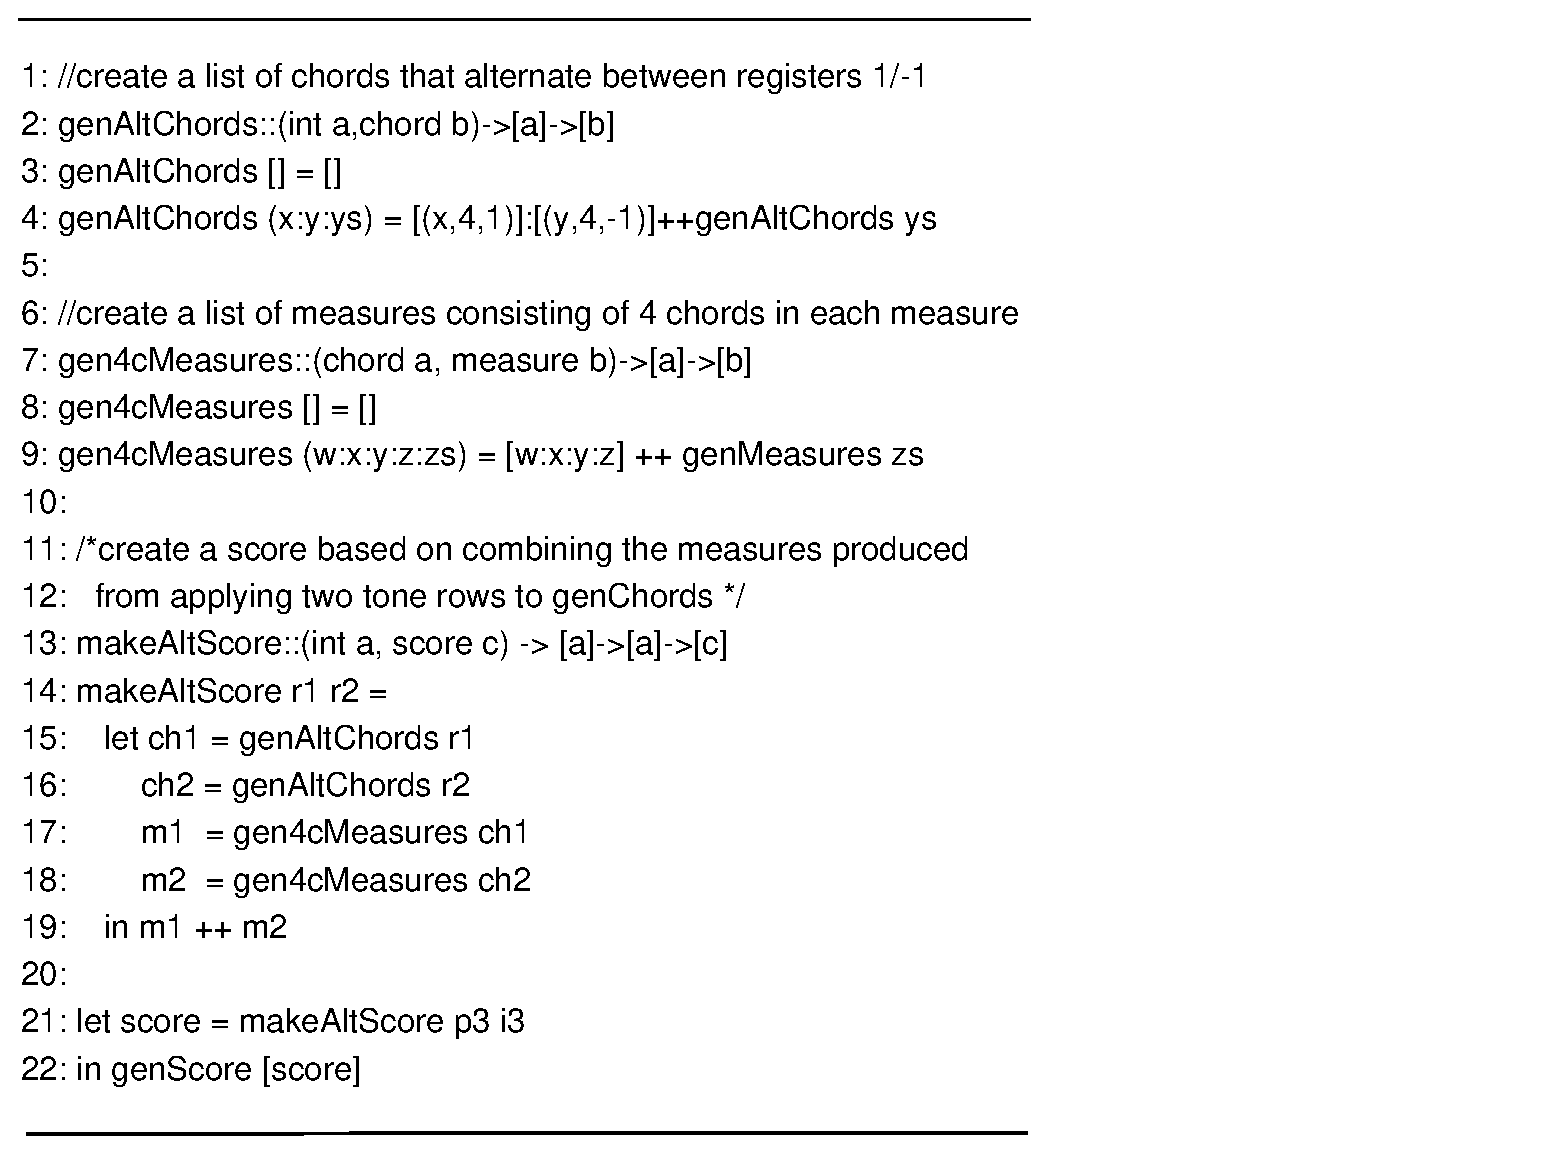
\includegraphics[width=\textwidth]{figures/example2}
  \caption{This SMURF code takes in the p3 and i3 tone rows from Figure~\ref{fig:example1} and generates a score consisting of notes that alternate between the -1 and 1 registers.}
  \label{fig:example2}
\end{figure}

% comment out
\iffalse
\small
\begin{verbatim}
1: prime = [0,2,4,6,8,10,1,3,5,7,9,11]
2: p3    = trans 3 prime
3: i3    = inver p3
4: ri3   = rev i3
5: firstNotes = rowToNotes ri3 [4,4,4,4,4,4,4,4,4,4,4,4] [0,0,0,0,0,0,0,0,0,0,0,0]
6: firstMeasure = head firstNotes:(head (tail firstNotes)):(-1,4,0):(-1,4,0):[]
7: genScore [firstMeasure]
\end{verbatim}

\small
\begin{verbatim}
1: //create a list of chords that alternate between registers 1/-1
2: genAltChords::(int a,chord b)->[a]->[b]
3: genAltChords [] = []
4: genAltChords (x:y:ys) = [(x,4,1)]:[(y,4,-1)]++genAltChords ys
5: 
6: //create a list of measures consisting of 4 chords in each measure
7: gen4cMeasures::(chord a, measure b)->[a]->[b]
8: gen4cMeasures [] = []
9: gen4cMeasures (w:x:y:z:zs) = [w:x:y:z] ++ genMeasures zs
10:
11: /*create a score based on combining the measures produced
12:   from applying two tone rows to genChords */
13: makeAltScore::(int a, score c) -> [a]->[a]->[c]
14: makeAltScore r1 r2 = 
15:    let ch1 = genAltChords r1
16:        ch2 = genAltChords r2
17:        m1  = gen4cMeasures ch1
18:        m2  = gen4cMeasures ch2
19:    in m1 ++ m2 
20:
21: let score = makeAltScore p3 i3 
22: in genScore [score]
\end{verbatim}
\fi
